%
% File acl2020.tex
%
%% Based on the style files for ACL 2020, which were
%% Based on the style files for ACL 2018, NAACL 2018/19, which were
%% Based on the style files for ACL-2015, with some improvements
%%  taken from the NAACL-2016 style
%% Based on the style files for ACL-2014, which were, in turn,
%% based on ACL-2013, ACL-2012, ACL-2011, ACL-2010, ACL-IJCNLP-2009,
%% EACL-2009, IJCNLP-2008...
%% Based on the style files for EACL 2006 by 
%%e.agirre@ehu.es or Sergi.Balari@uab.es
%% and that of ACL 08 by Joakim Nivre and Noah Smith

\documentclass[11pt,a4paper]{article}
\usepackage[hyperref]{acl2020}
\usepackage{booktabs}
\usepackage{graphicx}
\usepackage{times}
\usepackage{latexsym}
\usepackage{multirow}
\renewcommand{\UrlFont}{\ttfamily\small}

\usepackage{microtype}

\aclfinalcopy % Uncomment this line for the final submission


\newcommand\BibTeX{B\textsc{ib}\TeX}

\title{OT$^3$P: Optimal-Transport guided Test-Time Adaptation for Vision-Language Models}

\author{Yunbei Zhang \\
  Tulane University / New Orleans, LA \\
  \texttt{yzhang111@tualne.edu} \\\And
  Janet Wang \\
  Tulane University / New Orleans, LA \\
  \texttt{swang47@tulane.edu} \\}

\date{}

\begin{document}
\maketitle
\begin{abstract}
  We propose a novel algorithm for Test-Time Adaptation (TTA), Optimal Transport-guided Test-Time Visual Prompting (OT-VP), for Language and Vision-Language models.
  This method aims to enhance the performance of pre-trained models when applied to previously unseen target tasks. 
  Specifically, OT-VP employs Optimal Transport (OT) distance to learn a universal visual prompt, effectively aligning the distribution of the unseen target data with the source distribution, thereby facilitating more accurate model predictions. 
  Upon evaluation, our approach demonstrates a significant improvement in accuracy. 

\end{abstract}


\section{Introduction}

The remarkable successes of Deep Neural Networks (DNNs) are often tempered by the challenges posed by discrepancies between training and testing data distributions \cite{recht2019imagenet, hendrycks2019benchmarking, koh2021wilds}.
Such discrepancies are not uncommon in real-world applications, where variations in data due to natural differences and stylistic changes can significantly impact model performance \cite{ li2017deeper}.
This problem has been well-documented across various studies, underscoring the fragility of DNNs in the face of distribution shifts \cite{hendrycks2019benchmarking}. 
Domain Generalization (DG) has been proposed as a solution to this challenge, aiming to equip models with the ability to generalize to unseen domains by leveraging information from source domains during the training phase \cite{blanchard2011generalizing, zhou2022domain}. 
Despite considerable efforts in this area, machine learning systems remain susceptible to domain shifts, with studies indicating minimal performance gains over conventional Empirical Risk Minimization (ERM) approaches \cite{gulrajani2020search, mehra2022do}.

In response to these limitations, a new line of research has emerged, focusing on enhancing model performance directly at test time \cite{wang2021tent, NEURIPS2021_1415fe9f}. 
This approach allows models to leverage unlabeled test data from target domains. 
This data offers insights into the target distribution, insights that are typically inaccessible in the DG framework. 
Test-time adaptation, as demonstrated in \cite{NEURIPS2021_1415fe9f}, surpasses the capabilities of many existing DG strategies by utilizing immediate, real-world data to refine model accuracy.
Inspired by these insights, our work pivots towards exploring test-time adaptation (TTA) as a strategic response to the challenges of domain shifts, aiming to harness the full potential of DNNs in unseen environments. Our motivations shows in Fig. \ref{fig:motivation}

\begin{figure}[t]
    \centering
    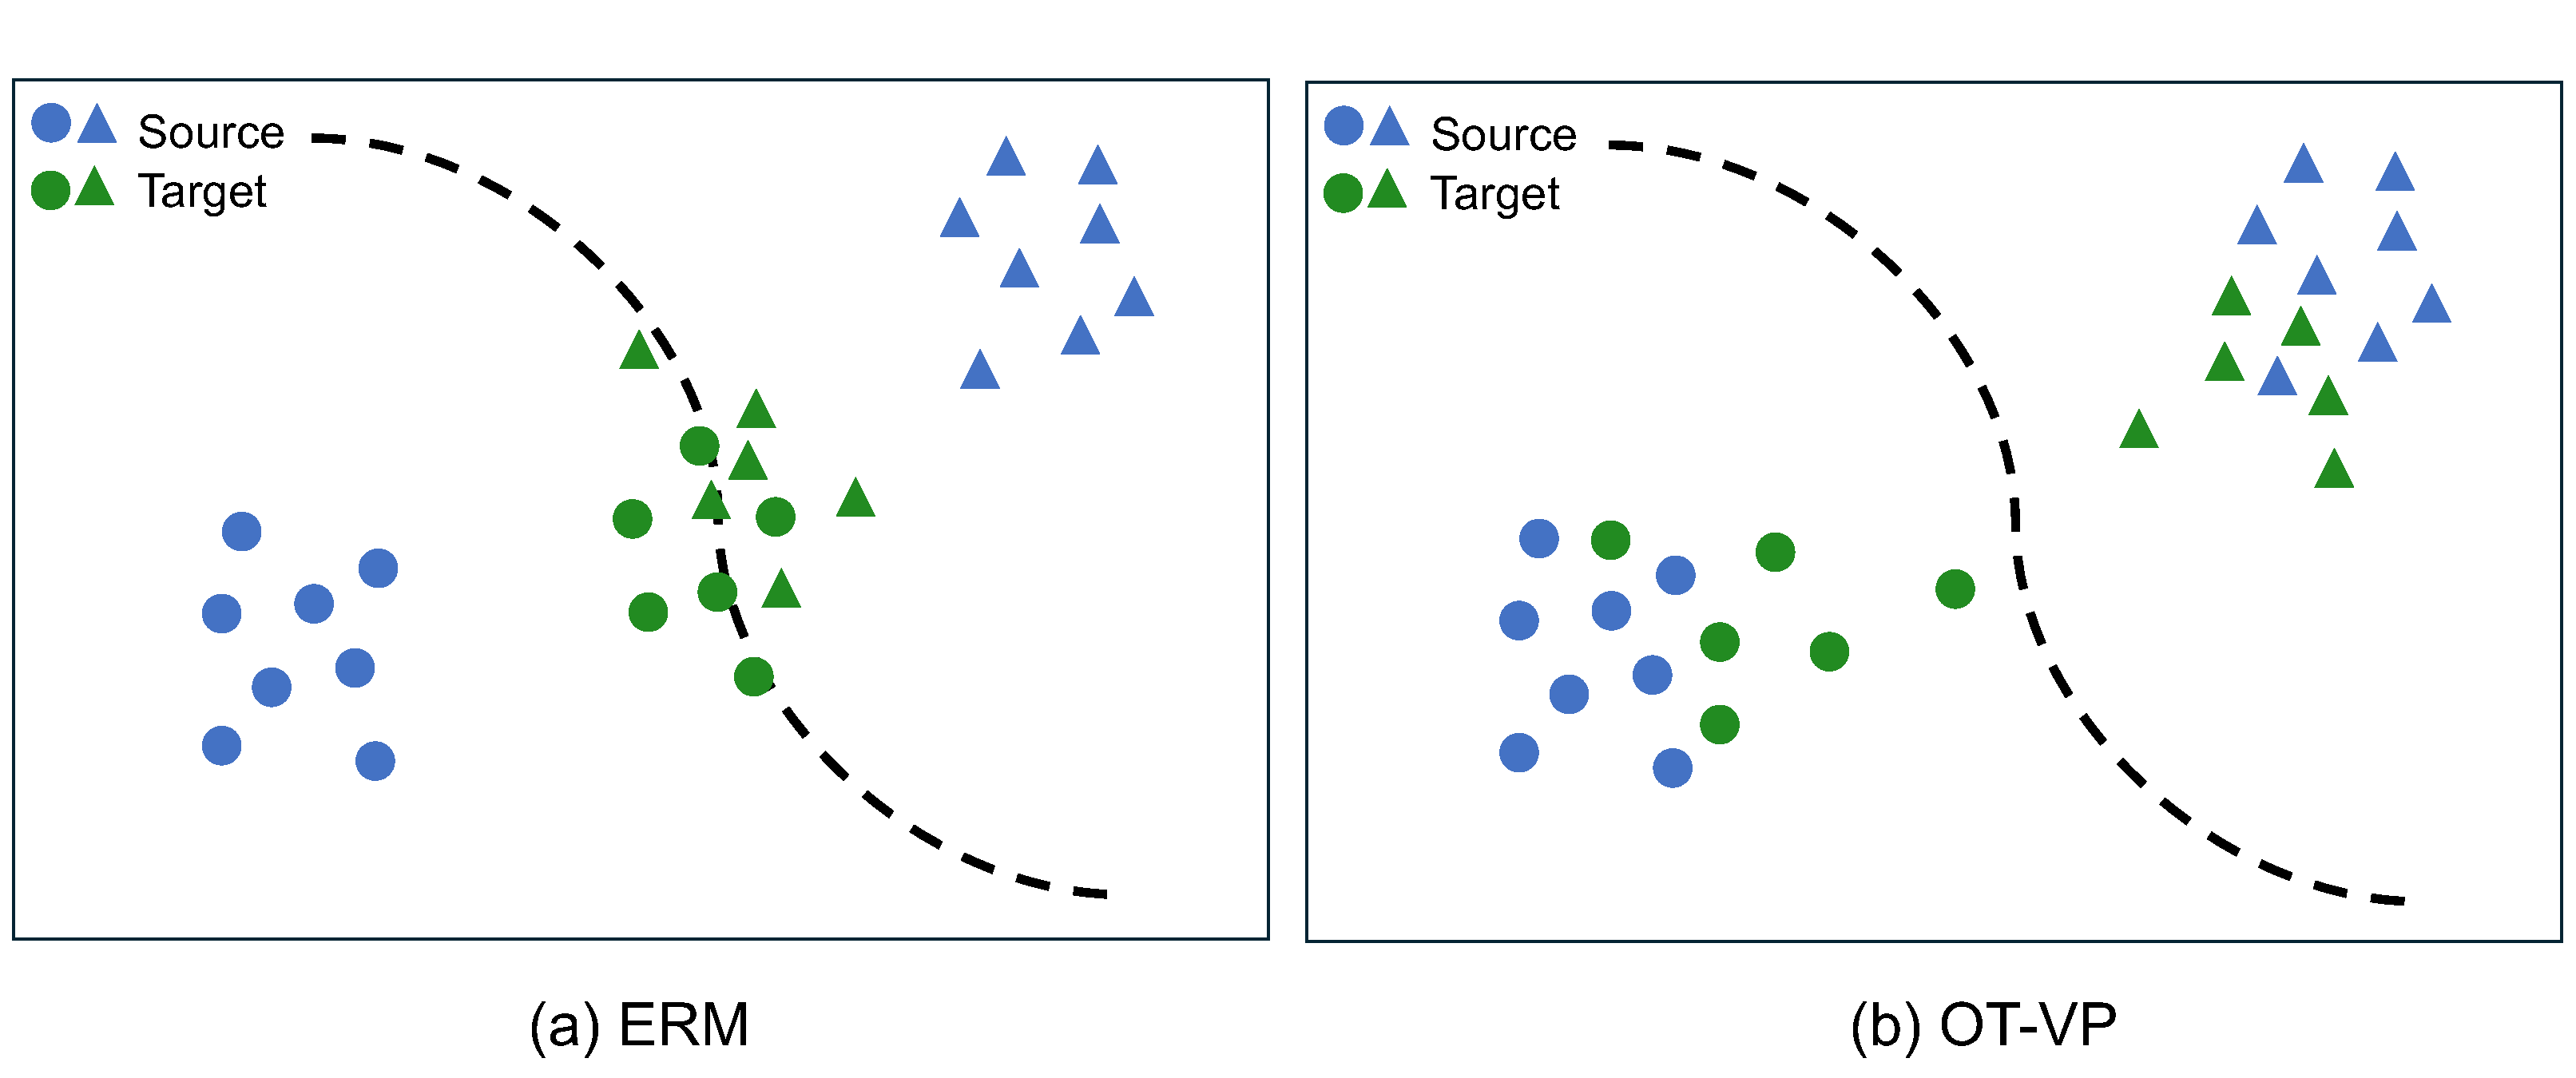
\includegraphics[width=1\linewidth]{motivation.pdf}
    \caption{Motivation of our approach. (a) An ERM model trained on the source domain struggles to adapt to the target domain due to domain shifts. (b) Our method optimizes prompt tokens by minimizing the Optimal Transport distance to align the target domain with the source domain without changing the decision boundary.
    }
    \label{fig:motivation}
    \vspace{-0.5cm}
\end{figure}

\section{Related Work}

\textbf{Optimal Transport} Optimal Transport (OT) theory, tracing back to the Monge problem in 1781, evolved significantly with the introduction of the Kantorovich relaxation \cite{kantorovich1942translocation} in 1942. 
This advancement transformed OT into a robust framework for comparing distributions, shapes, and point clouds \cite{peyre2019computational}, leveraging the geometry of the underlying space. 
OT operates on a complete and separable metric space $\mathcal{X}$, utilizing continuous or discrete probability measures $P, Q \in \mathcal{P(X)}$. 
The Kantorovich formulation defines the OT problem as:
\begin{equation}
\mathrm{OT}_c(P, Q) := \mathop{\inf}\limits_{\pi \in \Pi(P, Q)} \int_{\mathcal{X} \times \mathcal{X}} c(\mathbf{x}_1, \mathbf{x}_2)d\pi (\mathbf{x}_1, \mathbf{x}_2),
\end{equation}
where $c(\cdot,\cdot): \mathcal{X}\times\mathcal{X} \rightarrow \mathbb{R^+}$ denotes a cost function, and $\Pi(P, Q)$ represents the set of all possible couplings or joint distributions over $\mathcal{X}\times\mathcal{X}$ with $P$ and $Q$ as their marginals. 
The term $W_p(P,Q) := \mathrm{OT}_c(P, Q)^{\frac{1}{p} }$ is referred to as the $p$-Wasserstein distance when the cost function $c(\mathbf{x}_1, \mathbf{x}_2)=d(\mathbf{x}_1, \mathbf{x}_2)^p$ for some $p\geq1$ where $d$ is a metric of $\mathcal{X}$.

In real-world applications, the true marginal distributions $P, Q$ are often unknown, leading to reliance on discrete empirical distributions $\hat{P}=\sum_{i=1}^{m}\mathbf{a}_i\delta_{\mathbf{x}_1^i}$ and $\hat{Q}=\sum_{i=1}^{n}\mathbf{b}_i\delta_{\mathbf{x}_2^i}$, with $\mathbf{a},\mathbf{b}$ as vectors in the probability simplex. 
The cost function then simplifies to an $m \times n$ cost matrix $\mathbf{C}$, where $\mathbf{C}_{ij} = c(\mathbf{x}_1^i, \mathbf{x}_2^j)$. 
For computational efficiency, the Sinkhorn algorithm \cite{cuturi2013sinkhorn} introduces an entropic regularizer to the OT problem, facilitating practical applications such as domain adaptation \cite{courty2016optimal} and the evaluation of distances between datasets \cite{alvarez2020geometric}. 
This regularized approach, which can be computed using \verb|POT| \cite{flamary2021pot}, allows for the computation of an optimal mapping from source to target domains.


\section{Methods}

\subsection{Preliminaries}
\label{problem_setup_preliminaries}
\textbf{Problem Definitions} Denote the source (target) domain as $\mathcal{D}^s=\{\mathbf{x}_i^s, y_i^s\}_{i=1}^{n_s}$ ($\mathcal{D}^t=\{\mathbf{x}_i^t, y_i^t\}_{i=1}^{n_t}$, where $\mathbf{x} \in \mathcal{X}$ represents the input image and $y\in \mathcal{Y}$ is the label.
The dataset $\mathcal{D}^s$ ($\mathcal{D}^t$) comprises samples that are identically and independently distributed (i.i.d.), characterized by some probability distribution $P^s(X, Y)$ ($P^t(X, Y)$).

In the context of Test-Time Adaptation (TTA), the model $f$ is initially trained on the source domain, e.g. minimizing the empirical risk, 
\begin{equation}
\label{eq:erm}
    \mathop{\arg \min}\limits_{f} \frac{1}{n_s} \sum_{i=1}^{n_s} \ell(f(\mathbf{x}_i^s), y^s)
\end{equation}
where $\ell$ is a loss function. Throughout this paper, we refer to optimizing the model with Eq. \ref{eq:erm} as ERM. 
Generally, the model $f$ is structured as a composition $h \circ \phi$, with the feature extractor $\phi: \mathcal{X} \rightarrow \mathcal{Z}$ learning the input's representation, and the classifier $h: \mathcal{Z} \rightarrow \mathcal{Y}$ predicting the class label. 

For any unlabelled target domain $\mathcal{D}^t$, TTA aims to adapt model $f$ or/and target input $x^t$ to bridge the performance gap under the assumption that the source domain and target domain share the same label set. In our approach, we employ a Vision Transformer as the model $f$, which remains fixed during adaptation.

\subsection{Test-time Adaptation with OT$^3$P}
\label{ot-vp}
In the test-time scenario, labeled target data is not available, thereby the prompt cannot be optimized. 
Thus, we propose an unsupervised prompt adaptation method: Optimal Transport-guided Test-Time Visual Prompt Adaptation (OT-VP). 

Given an unlabelled target dataset $\mathcal{D}^t$, we pass them through the visual encoder with learnable prompts to get the representation. 
Source representations are computed offline and utilized directly at test time. 
Then we compute the OT distance between source and target representations. 
Here, we consider two cost functions for OT: The first is the cost between two representations without label information, i.e., for any two representations $\mathbf{z}^s$, $\mathbf{z}^t$, 
\begin{equation}
    c(\mathbf{z}^s, \mathbf{z}^t) = \|\mathbf{z}^s- \mathbf{z}^t||_2
\end{equation}

The other includes label/pseudo-label information:
\begin{equation}
    c((\mathbf{z}^s, y^s), (\mathbf{z}^t, \hat y^t)) = \|\mathbf{z}^s- \mathbf{z}^t||_2 + \infty \cdot \mathbbm{1}_{\{y^s \neq \hat y^t\}}
\end{equation}
where $\hat y^t$ is the pseudo label from the pre-trained model.
The OT distance will be used to update the prompts for the target dataset as follows:
\begin{equation}
\label{eq:ot-vp}
    \mathbf{\gamma}^* = \mathop{\arg \min}\limits_{\mathbb{\gamma}} OT_c(P^s_\#, P^t_\#)
\end{equation}
where $P^s_\#$ is a distribution over $(\phi(\mathbf{x}^s), y^s)$ and $P^t_\#$ is a distribution over $(\phi(\mathbf{x}^t), \hat y^t)$ with pseudo label $\hat y^t := f(\mathbf{x}^t; \mathbf{\gamma}))$

\subsection{Vision Transformers}
\label{sec:vit}
A Vision Transformer (ViT) \cite{dosovitskiy2021an, liu2021swin} processes an input image $x$ by initially dividing it into $k$ patches $\{I_i\}_{i=1}^k$. 
An encoding layer $E$ is employed to transform the input patches into patch tokens, to which positional embedding are subsequently added to retain spatial information. 
The inputs to the transformer layers consist of these encoded patch tokens augmented with a special classification token \verb|[CLS]|. 
The ViT is composed of several sequential blocks, and each block contains an attention layer and a Multi-Layer Perceptron  (MLP) layer. 
The prediction of the vision transformer can be formulated as follows:
\begin{equation}
\begin{aligned}
    \texttt{[CLS]} &= \phi([\texttt{[CLS]}, E(I_1), ..., E(I_k)]), \\
    y &= h(\texttt{[CLS]}),
\end{aligned}
\end{equation}
where $[\cdot]$ represents concatenation of tokens. 

Incorporating a visual prompt into the ViT represents a parameter-efficient approach for fine-tuning or adapting the model, particularly when it is fixed \cite{jia2022visual, ge2023domain}. 
By introducing $l$ prompt tokens $\{\texttt{[Prompt]}_i\}_{i=1}^l=: \mathbf{\gamma}$, the prediction process can be reformulated as follows:
\begin{equation}
\begin{aligned}
    \texttt{[CLS]} &= \phi([\texttt{[CLS]}, \{E(I_i)\}_{i=1}^k, \gamma]) \\
    y &= h(\texttt{[CLS]})
\end{aligned}
\label{eq:infer_with_prompt}
\end{equation}
The optimal prompts can be optimized as follows when the labels are available:
\begin{equation}
\label{eq:supervised_vp}
    \mathbf{\gamma}^* = \mathop{\arg \min}\limits_{\mathbf{\gamma}} \mathbb{E}[\ell(f(\mathbf{x}; \mathbb{\gamma}), y)]
\end{equation}

\subsection{Optimal Transport}
\label{sec:ot}
Optimal Transport (OT) theory, tracing back to the Monge problem in 1781, evolved significantly with the introduction of the Kantorovich relaxation \cite{kantorovich1942translocation} in 1942. 
This advancement transformed OT into a robust framework for comparing distributions, shapes, and point clouds \cite{peyre2019computational}, leveraging the geometry of the underlying space. 
OT operates on a complete and separable metric space $\mathcal{X}$, utilizing continuous or discrete probability measures $P, Q \in \mathcal{P(X)}$. 
The Kantorovich formulation defines the OT problem as:
\begin{equation}
\mathrm{OT}_c(P, Q) := \mathop{\inf}\limits_{\pi \in \Pi(P, Q)} \int_{\mathcal{X} \times \mathcal{X}} c(\mathbf{x}_1, \mathbf{x}_2)d\pi (\mathbf{x}_1, \mathbf{x}_2),
\end{equation}
where $c(\cdot,\cdot): \mathcal{X}\times\mathcal{X} \rightarrow \mathbb{R^+}$ denotes a cost function, and $\Pi(P, Q)$ represents the set of all possible couplings or joint distributions over $\mathcal{X}\times\mathcal{X}$ with $P$ and $Q$ as their marginals. 
The term $W_p(P,Q) := \mathrm{OT}_c(P, Q)^{\frac{1}{p} }$ is referred to as the $p$-Wasserstein distance when the cost function $c(\mathbf{x}_1, \mathbf{x}_2)=d(\mathbf{x}_1, \mathbf{x}_2)^p$ for some $p\geq1$ where $d$ is a metric of $\mathcal{X}$.

In real-world applications, the true marginal distributions $P, Q$ are often unknown, leading to reliance on discrete empirical distributions $\hat{P}=\sum_{i=1}^{m}\mathbf{a}_i\delta_{\mathbf{x}_1^i}$ and $\hat{Q}=\sum_{i=1}^{n}\mathbf{b}_i\delta_{\mathbf{x}_2^i}$, with $\mathbf{a},\mathbf{b}$ as vectors in the probability simplex. 
The cost function then simplifies to an $m \times n$ cost matrix $\mathbf{C}$, where $\mathbf{C}_{ij} = c(\mathbf{x}_1^i, \mathbf{x}_2^j)$. 
For computational efficiency, the Sinkhorn algorithm \cite{cuturi2013sinkhorn} introduces an entropic regularizer to the OT problem, facilitating practical applications such as domain adaptation \cite{courty2016optimal} and the evaluation of distances between datasets \cite{alvarez2020geometric}. 
This regularized approach, which can be computed using \verb|POT| \cite{flamary2021pot}, allows for the computation of an optimal mapping from source to target domains.


\section{Results}
For the purpose of computational efficiency, we employ simplified versions of the pre-trained BERT and RoBERTa models \cite{sanh2020distilbert}. We focus on two datasets, Stanford Sentiment Treebank (SST) and Yelp \cite{zhang2015character}, each containing five distinct classes. Our baseline approach, denoted as Empirical Risk Minimization (ERM), involves using one of these datasets as the source domain for fine-tuning the pre-trained model, followed by evaluation on the other dataset to assess transferability. Our proposed method introduces the concept of learning prompt tokens tailored to the target task subsequent to the initial pre-training phase. Furthermore, we conduct a comparative analysis with the current Test-Time Adaptation (TTA) method, known as Tent \cite{wang2021tent}, to evaluate the efficacy of our approach.

Table \ref{tab:main} demonstrates our method across different pre-trained models and target tasks. Table \ref{tab:main1} show the comparison between our method and SOTA on CLIP models.

\begin{table}[ht]
\centering

\begin{tabular}{lccc}
\hline
\textbf{Model} & \textbf{Algorithm} & \textbf{SST} & \textbf{Yelp} \\
\hline
\multirow{3}{*}{\textbf{BERT}} & ERM & 34.8 & 37.3 \\
& Tent & 41.2 & 43.5 \\
& OT$^3$P & 47.2 & 49.3 \\
\hline

\multirow{3}{*}{\textbf{RoBERTa}} & ERM & 35.1 & 36.3 \\
& Tent & 46.7 & 41.5 \\
& OT$^3$P & 51.3 & 48.7 \\
\hline

\end{tabular}
\caption{\label{tab:a_table} Comparison of Algorithm Performance on Sentiment Analysis for the Target Domain}
\label{tab:main}
\end{table}

\begin{table}[ht]
\centering
\begin{tabular}{lccccc}
\hline
\textbf{Algorithm} & \textbf{ImageNet V2} & \textbf{ImageNet Sketch} & \textbf{ImageNet A} & \textbf{ImageNet R} & \textbf{OOD Avg.} \\
\hline
\textbf{MaPLe} & 64.07 & 49.15 & 50.90 & 76.98 & 60.28 \\
 \textbf{MaPLe+TPT} & 64.87 & 48.16 & 58.08 & 78.12 & 62.31 \\
 \textbf{OT$^3$P} & 65.29 & 50.23 & 59.37 & 79.33 & 63.55 \\
\hline
\end{tabular}
\caption{Comparison of Algorithm Performance on Objective Detection Tasks for CLIP Model}
\label{tab:main1}
\end{table}


\section{Discussion and Conclusion}

We propose OT$^3$P, a novel test-time adaptation approach that leverages prompt learning for effective test-time adaptation. 
OT$^3$P stands out by adapting without altering the pre-trained model and effectively aligning the source and target domains, offering a more practical solution than established methods. 
Our experiments reveal OT$^3$P strengths: consistently outperforming existing TTA methods for ViT and DG prompt learning, and reducing prediction entropy to increase model confidence. By optimizing universal prompts for the target domain, OT$^3$P simplifies the adaptation process, enhancing the applicability of deep learning models in real-world settings.

% \section{Division of Labor}
% \begin{itemize}
%     \item Janet will be responsible for running the experiments, analyzing the experimental results, and writing the report. 
%     \item Yunbei will be responsible for collecting the data, surveying related works, and running the experiments.
% \end{itemize}


\clearpage
\newpage

\bibliography{references}
\bibliographystyle{acl_natbib}


\end{document}
